% Subsection on breadboard

Pour le prototypage de circuits électroniques, on utilise généralement une \emph{breadboard} (ou platine d'expérimentation/prototypage). Il s'agit d'une "plaquette à trous", dans lesquels on peut insérer des fils et des composants pour construire un petit circuit électronique. Un exemple de breadboard se trouve sur la Figure \ref{fig:breadboard_pic}.

Les trous d'une breadboard ne sont pas isolés les uns des autres, ils sont connectés en colonnes ou en lignes, comme illustré sur la Figure \ref{fig:breadboard_conn}. Généralement, les deux premières et les deux dernières colonnes de trous, assignés des signes + et -, sont utilisées pour distribuer les signaux d'alimentation (0V et 5V par exemple). Les lignes de trous au milieu sont plutôt utilisées pour connecter et placer le coeur du circuit.

Comme une breadboard ne nécessite aucune soudure, elle permet de prototyper et débugger rapidement un circuit électronique. Elle est également totalement réutilisable : si un circuit monté sur breadboard n'est plus utilisé, il peut être enlevé facilement en sortant les fils et composants des trous, et la breadboard peut alors être utilisée pour le prototypage d'un autre projet. La breadboard est donc très pratique, mais malheureusement, tous les composants ne peuvent pas y être connectés.\\

\begin{minipage}[t]{.49\textwidth}
	\centering
	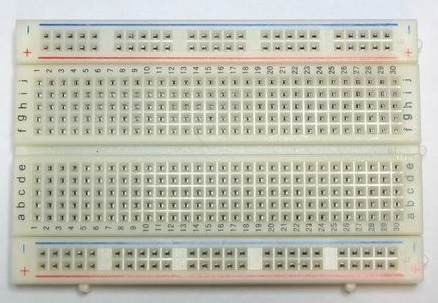
\includegraphics[width=.6\textwidth,angle=90]{figures/breadboard_picture.jpg}
	\captionof{figure}{Photo d'une breadboard.}
	\label{fig:breadboard_pic}
\end{minipage}
\hfill
\begin{minipage}[t]{.49\textwidth}
	\centering
	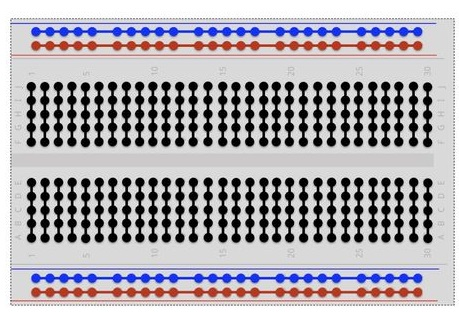
\includegraphics[width=.6\textwidth,angle=90]{figures/breadboard_connections.jpg}
	\captionof{figure}{Connexions des trous d'une breadboard.}
	\label{fig:breadboard_conn}
\end{minipage}
\vspace{1cm}